\documentclass[a4paper, titlepage]{article}
\usepackage[round, sort, numbers]{natbib}
\usepackage[utf8]{inputenc}
\usepackage{amsfonts, amsmath, amssymb, amsthm}
% \usepackage[scaled]{beramono}
\usepackage{color}
\usepackage{listings}
\usepackage{marvosym}
\usepackage{mathtools}
\usepackage{paralist}
\usepackage{parskip}
\usepackage{subfig}
\usepackage{tikz}
\usepackage{titlesec}

\numberwithin{figure}{section}
\numberwithin{table}{section}

\usetikzlibrary{arrows, automata, backgrounds, petri, positioning}
\tikzstyle{place}=[circle, draw=blue!50, fill=blue!20, thick]
\tikzstyle{transition}=[rectangle, draw=black!50, fill=black!20, thick]

\lstset{
  basicstyle=\ttfamily\small,
  columns=fullflexible,
  breaklines=true
}

% define new commands for sets and tuple
\newcommand{\setof}[1]{\ensuremath{\left \{ #1 \right \}}}
\newcommand{\tuple}[1]{\ensuremath{\left \langle #1 \right \rangle }}
\newcommand{\card}[1]{\ensuremath{\left \vert #1 \right \vert }}

\makeatletter
\newcommand\objective[1]{\def\@objective{#1}}
\newcommand{\makecustomtitle}{%
	\begin{center}
		\huge\@title \\
		[1ex]\small Aurélien Coet, Dimitri Racordon
	\end{center}
	\@objective
}
\makeatother

\begin{document}

\title{Outils formels de Modélisation \\ 6\textsuperscript{ème} séance d'exercices}
\author{Aurélien Coet, Dimitri Racordon}
\objective{%
Dans cette séance d'exercices, nous allons implémenter des procédures permettant de vérifier certaines propriétés classiques des réseaux de Petri.%
}

\makecustomtitle

\section{Implémentation [\Keyboard] ($\bigstar\bigstar$)}

Considérez le réseau de la figure \ref{fig:producer-consumer},
lequel représente un modèle \emph{producteur consommateur}.

\begin{enumerate}
  \item Ce réseau est-il bloquable ? 
  \item Ce réseau est-il vivant ?
  \item Ce réseau est-il réversible ?
  \item Donnez la définition (formelle) de ces propriétés.
\end{enumerate}

\begin{figure}[ht]
	\centering
  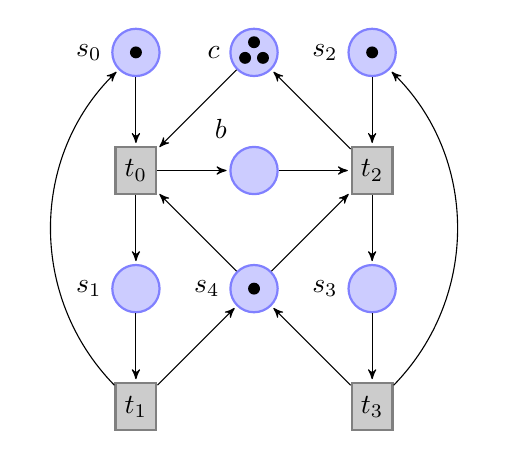
\begin{tikzpicture}[node distance=1.5cm, minimum height=6mm, >=stealth', bend angle=45, auto]
    \node[place,tokens=1] (s0) [label=left:$s_0$] {};
    \node[place]          (s1) [below of=s0, yshift=-1.5cm, label=left:$s_1$] {};

    \node[place,tokens=3] (cb) [right of=s0, label=left:$c$] {};
    \node[place]          (b)  [below of=cb, label=135:$b$] {};
    \node[place,tokens=1] (s4) [below of=b, label=left:$s_4$] {};

    \node[place,tokens=1] (s2) [right of=cb, label=left:$s_2$] {};
    \node[place]          (s3) [below of=s2, yshift=-1.5cm, label=left:$s_3$] {};

    \node [transition] (t0) [below of=s0] {$t_0$}
				  edge [pre]  (s0)
          edge [pre]  (cb)
          edge [pre]  (s4)
          edge [post] (b)
          edge [post] (s1);
    \node [transition] (t1) [below of=s1] {$t_1$}
				  edge [pre]  (s1)
          edge [post,bend left] (s0)
          edge [post] (s4);

    \node [transition] (t2) [below of=s2] {$t_2$}
				  edge [pre]  (s2)
          edge [pre]  (s4)
          edge [pre]  (b)
          edge [post] (cb)
          edge [post] (s3);
    \node [transition] (t3) [below of=s3] {$t_3$}
				  edge [pre]  (s3)
          edge [post,bend right] (s2)
          edge [post] (s4);
  \end{tikzpicture}
  \caption{Modèle d'un producteur-consommateur}
  \label{fig:producer-consumer}
\end{figure}

Complétez la définition des fonctions \texttt{isBlockable} et \texttt{isReversible} dans le fichier \texttt{Analysis.fs} du projet \texttt{Exercise}.
Vous pouvez vous inspirer de l'implémentation de la fonction \lstinline|isAlive|, définie dans le même fichier.

\section{Utilisation [\Keyboard] ($\bigstar\bigstar$)}

A l'aide des fonctions \lstinline|isBlockable|, \lstinline|isReversible| et \lstinline|isAlive|, tâchez de créer un réseau qui soit:

\begin{enumerate}
  \item Non-bloquable, réversible et vivant
  \item Non-bloquable, réversible et non-vivant
  \item Non-bloquable, non-réversible et non-vivant
  \item Bloquable, non-réversible et non-vivant
\end{enumerate}

\end{document}
